\chapter{Feature extraction}

In this chapter we will present necessary framework for feature extraction: basic signal processing ideas and finally the mel frequency cepstral coefficient (MFCC) extraction procedure. The MFCC is based on the early work of the \textcite{stevens_scale_1937} in which they makes assumption that frequency heard by human is in the logarithmic scale:

\begin{equation}
	\label{eq:mel}
	M(f) = 1127\log\left(1+\frac{f}{700}\right)
\end{equation}

\subsection{Digital Signal Processing}

Signal $x_a(t), -\infty < t < \infty$ is a~function of independent variable which is the time. In order to digitize signal and be able to store it into memory we must digitize signal and create sequence or a~function. The process is done using Analog Digital converter - device which converts analog to digital signal using a~sampler and a~quantizer.

The sampler ``takes samples'' of the analog signal $x_a(t)$ every $T_s$ seconds. The sampling frequency $F_s$, the sampling period, independent variable - time($t$) and independent variable - sample (n) are related by formula:

\begin{equation}
	t = nT_s = \frac{n}{F_s}
\end{equation}

\begin{equation}
	x_a(nT) \equiv x(n)
\end{equation}


Most often functions used in the signal analysis are cosine and sine waves in the form:
\begin{equation}
	x_a(t) = Acos(\Omega t +~\theta)
\end{equation}

\begin{equation}
	\Omega \equiv 2\pi F
\end{equation}

Where A~is an strength of the amplitude, $\Omega$ - frequency (rad/s), F - Hz, $\theta$ - phase (rad) shift.  
Similar we can define those variables in digital domain:

\begin{equation}
	x(n) = Acos(\omega t +~\theta)
\end{equation}

\begin{equation}
	\omega \equiv 2\pi f
\end{equation}


Where A~is an strength of the amplitued, $\omega$ - frequency (radians/sample), f - (cycles/sample), $\theta$ - phase (rad) shift.  

N~is a~period of the~signal when


\begin{align}
& x(n+N) = x(n), \forall n \in \mathbb{Z} \\
& cos(2\pi f (n +~N) +~\theta) = cos(2\pi f n +~\theta) \\
& f = \frac{k}{N}, k \in \mathbb{Z} \implies f \in \mathbb{Q}
\end{align}
This implies that frequency in digital time domain is a rational number.  

Equation:
\begin{equation}
	x_k(n)=Acos(2\pi f_0(n) +~\theta),
\label{cosine_digital}
\end{equation}
is periodic, where period of $x_k$ equals


\begin{equation}
	2 \pi f = 2 \pi f_o +~2\pi k \implies f = f_0 + k, k \in \mathbb{N}
\end{equation}
This allow to distinguish range for fundamental frequency $f_0$
\begin{equation}
|f_0| < \frac{1}{2}
\label{fundamental_one_half}
\end{equation}
Frequencies $|f| > \frac{1}{2}$ are called ``alias frequencies'' which ``mirror'' the~fundamental frequency from range $f_0$.


When we sample an analog cosine signal $x_a$ with the sampling frequency $F_s$, we get:

\begin{equation}
x_a(nT)=x_a(\frac{n}{F_s}) \equiv x(n) = Acos(\frac{2\pi n F}{F_s} +~\theta) 
\label{eq:cosine_sampling}
\end{equation}

Comparison of equations \eqref{eq:cosine_sampling} and \eqref{cosine_digital} yields 

\begin{equation}
f_0 = \frac{F}{Fs}
\label{fundamental_sampling}
\end{equation}

Substituting $f_0$ in \eqref{fundamental_one_half} by \eqref{fundamental_sampling} results in one of the most important conclusions in digital signal processing which is maximum frequency one can digitize:

\begin{equation}
	\abs*{\frac{F}{F_s}} < \frac{1}{2} \implies \abs{F} < \frac{F_s}{2}
\end{equation}
 

Maximum frequency which could be converted to digital domain is half of the sampling frequency - is called ``folding frequency'' $F_{fold}$. On the other hand having maximum frequency $F_{max}$ in our signal $x_a$ one is able to define ``Nyquist rate'', which is equal to $2 F_{max}$. Human ear is working in range $20 Hz <~F_h <~20kHz$, which yields ``Nyquist rate'' - the sampling frequency - 40kHz (often used frequency 44.1kHz due to imperfection of low\dywiz band filters). Speech lies in the range $< 16kHz$. Other frequencies $> 16kHz$ should be filtered\dywiz out by analog low\dywiz band filters. This subject is out of the scope of this work. 
`
An input signal is analog data which contains continuous range of values, therefore it should be quantize to fit into memory range. Quantization error should be introduced, because of quantizer ($Q[x(n)] \equiv x_q(n)$):

\begin{equation}
e_q(n) = x_q(n) - x(n)
\end{equation}

The problem can be solved by rounding or by truncation. In this work we will focus only on rounding. Error $e_q(n)$ is limited to:


\begin{equation}
	-\frac{\Delta}{2} < e_q(n) < \frac{\Delta}{2}
\end{equation}
where $\Delta$ means:

\begin{equation}
	\Delta = \frac{x_{max}-x_{min}}{L-1}
\end{equation}
where $x_{max}, x_{min}$ are the maximum and minimum values of the signal, L~is the number of quantization levels.

\begin{figure}[h]
\label{f:ala_ma_kota}
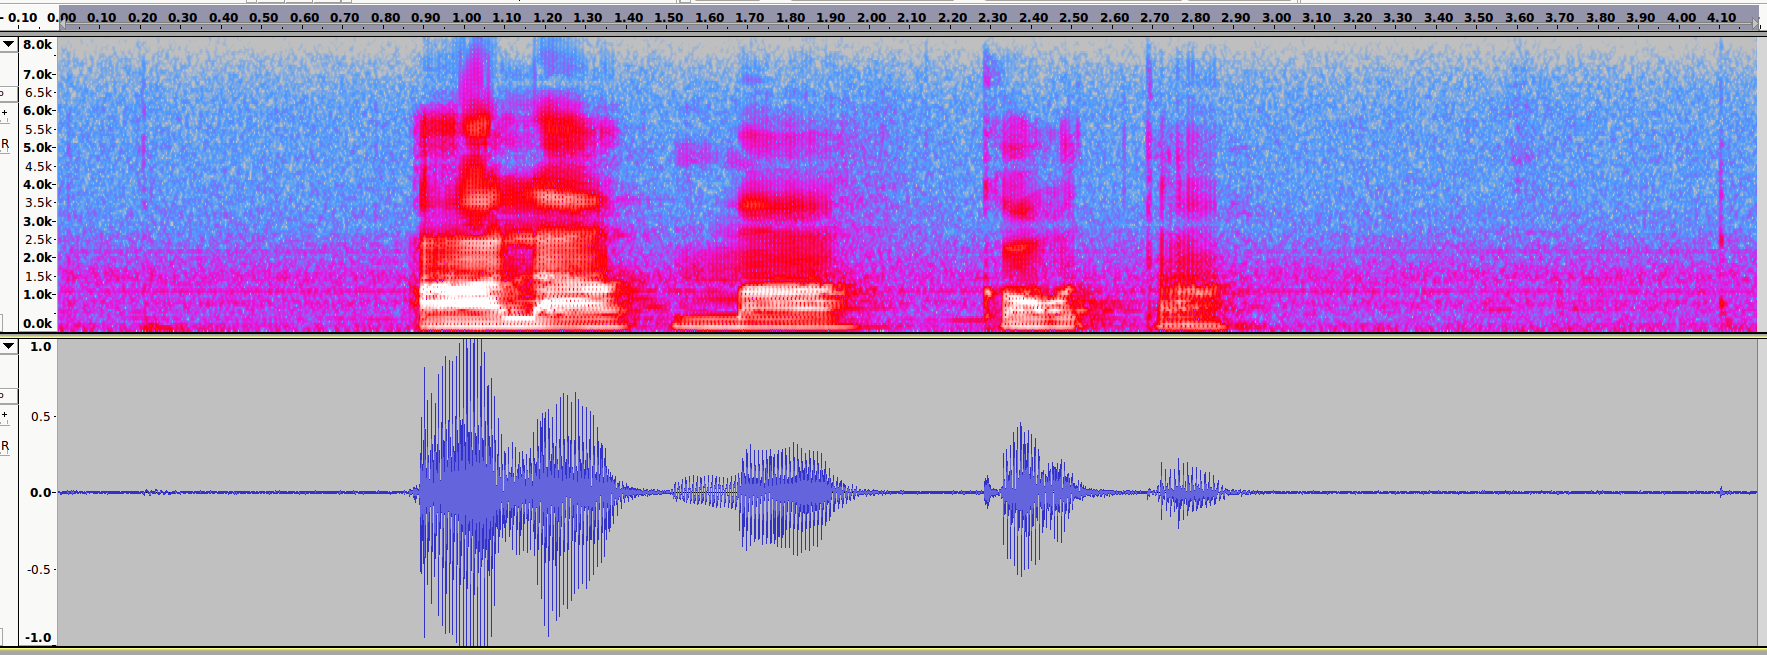
\includegraphics[width=\textwidth]{ala_ma_kota}
\caption{Example sentence in polish: ``Ala ma kota``. Time and frequency dimensions.}
\end{figure}

\section{MFCC}

Computations required for delta MFCC features consists of 7 steps \parencite{muda_voice_2010}. 

\begin{enumerate}
	\item Pre-emphasis: \\
		\begin{equation}
			y[n]=x[n]-0.95x[n-1]
		\end{equation}
		In this step we are raising energy of the signal at the higher frequencies.
	\item Framing: \\
		Signal is divided into overlapping segments with the size expressed as the frame size and the offset between edges called the frame shift. Default values for the frame size are 25 ms and for the frame shift 10 ms. For example in $16kHz$ signal in 1 second there are about 160 frames.
	\item Windowing: \\
		Because there is high probability that our signal is not period during our frame time (25s), when using frames one should use a window which change input response. The most common used window is hamming window as is the best for ``the closely space sine waves'' \parencite{national_instruments_understanding_????}:
\begin{equation}
	w(n)=0.54-0.46 \cos\left(\frac{2\pi n}{N-1} \right) \ 0 \le n \le N - 1
\end{equation}\
Using rectangular window leads to ``spectral leakages'' which put some power of the main lobe to the side lobs.	
	\item Fast Fourier Transform (FFT):
		Human inner ear is working the frequency space \parencite{jurafsky} instead of the time space, so we should move signal to the z space with discrete fourier transform (DFT): 
	\begin{equation}
		X[k]= \sum\limits^{N-1}_{n=0} x[n]\exp\left(\frac{-j2\pi kn}{N} \right), \ k=0,\ldots,N-1
	\end{equation}
	Figure \ref{f:ala_ma_kota} presents signal after FFT step.
		
	\item Mel filter bank:
		$K=40, F()$ triangular bandpass filters in the range $0,\ldots,8\text{kHz}$ are created uniformly on the mel scale. Then filters should be applied to the output of the FFT. Computations are quite complex (upper and lower frequencies on the mel scale), but can be found in the book of \textcite{huang_spoken_2001}. After this is process, logarithm is taken from filter banks. Those features are called Fbank features and often used in speech recognition.
	\item Inverse Discrete Fourier Transform (IDFT):  \\
		Speech signal $s[n]$ consists of the glottal excitation $u[n]$ convolved with the vocal tract $v[n]$:

		\begin{align}
		& s[n]=u[n] \star v[n] \\
		& S[n]=U[n]V[n] \\
		& \log |S[n]|= \log |U[n]| + \log |V[n]| 
		\end{align}

		\begin{equation}
			c[k]= \sum\limits^{N-1}_{n=0} \log \left( \sum\limits^{N-1}_{n=0} F(n)\exp\left(\frac{-j2\pi kn}{N} \right) \right) \exp\left(\frac{j2\pi kn}{N} \right), 
		\end{equation}

		Using logarithm and IDFT we are able to separate glottal excitation (high frequency harmonics) and vocal tract (low frequency harmonics). Additionally it changes periodicity of the signal in the frequency space. Small indexes of cepstral mel coefficients indicate vocal tract and high indexes of MFCC can show pitch (useful in accent recognition). In standard procedure we are using only 13 first coefficients.

	\item Deltas and Energy:
	\begin{equation}
		E = \suml_{t=t_0}^{t_N} x^2[t]
	\end{equation}

	Delta features:
	\begin{equation}
		d(t)=\frac{c(t+1)-c(t-1)}{2}	
	\end{equation}
	Double delta features:
	\begin{equation}
		d2(t)=\frac{d(t+1)-d(t-1)}{2}	
	\end{equation}

\section{Summary}

In this section we describe all techniques, which we are using in our experiments. Number of coefficients in kaldi scripts differ from those described by \textcite{jurafsky}. Our scripts are using:

\begin{itemize}
	\item 13 cepstral coefficients
	\item 13 delta cepstral coefficients 
	\item 13 double delta cepstral coefficients
	\item 1 energy coefficients
\end{itemize}






\end{enumerate}


